
\documentclass[12pt]{standalone}
\usepackage{tikz}
\usetikzlibrary{automata,positioning}
\begin{document}
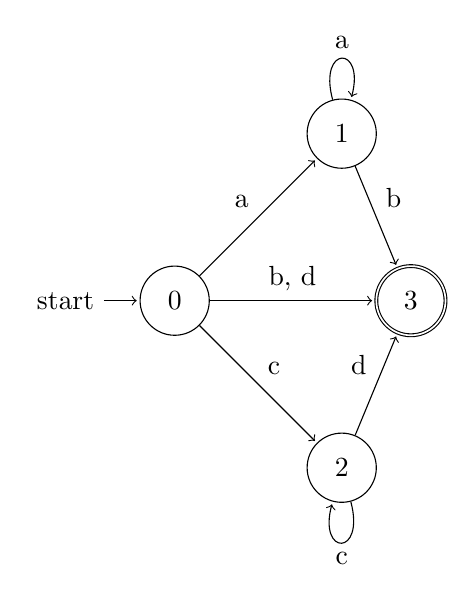
\begin{tikzpicture}[shorten >=1pt,node distance=3cm,on grid,auto] 
   \node[state, initial] (0) {$0$}; 
   \node[state] (1) [above right=of 0] {$1$};
   \node[state] (2) [below right=of 0] {$2$};
    \node[state, accepting] (3) [right=of 0] {$3$};

    \path[->] (0) edge  node {a} (1);
    \path[->] (0) edge  node {c} (2);
    \path[->] (0) edge  node {b, d} (3);

    \path[->] (1) edge [loop above] node  {a} (1);
    \path[->] (1) edge node {b} (3);
    
    \path[->] (2) edge [loop below] node  {c} (2);
    \path[->] (2) edge node {d} (3);
\end{tikzpicture}
\end{document}  

